% !TEX TS-program = xelatex
% !TEX encoding = UTF-8 Unicode
% !Mode:: "TeX:UTF-8"

%This file contains the LaTeX code of my laboratory report for my Database course.
%Author: 周芯怡/Xinyi Zhou <17307130354@fudan.edu.cn>
%Author: 张作柏/Zuobai Zhang <17300240035@fudan.edu.cn>


% This is a simple template for a LaTeX document using the "article" class.
% See "book", "report", "letter" for other types of document.

\documentclass[12pt]{article} % use larger type; default would be 10pt

\usepackage[utf8]{inputenc} % set input encoding (not needed with XeLaTeX)

%%% Examples of Article customizations
% These packages are optional, depending whether you want the features they provide.
% See the LaTeX Companion or other references for full information.

%%% PAGE DIMENSIONS
\usepackage[top=1.05in, bottom=0.95in, left=0.90in, right=1.10in]{geometry}
%\usepackage{geometry} % to change the page dimensions
\geometry{a4paper} % or letterpaper (US) or a5paper or....
% \geometry{margin=2in} % for example, change the margins to 2 inches all round
% \geometry{landscape} % set up the page for landscape
%   read geometry.pdf for detailed page layout information

\usepackage{graphicx} % support the \includegraphics command and options

% \usepackage[parfill]{parskip} % Activate to begin paragraphs with an empty line rather than an indent

%%% PACKAGES
\usepackage{booktabs} % for much better looking tables
\usepackage{array} % for better arrays (eg matrices) in maths
\usepackage{paralist} % very flexible & customisable lists (eg. enumerate/itemize, etc.)
\usepackage{verbatim} % adds environment for commenting out blocks of text & for better verbatim
%\usepackage{subfig} % make it possible to include more than one captioned figure/table in a single float
% These packages are all incorporated in the memoir class to one degree or another...

%%% HEADERS & FOOTERS
\usepackage{fancyhdr} % This should be set AFTER setting up the page geometry
\pagestyle{fancy} % options: empty , plain , fancy
%\renewcommand{\headrulewidth}{0pt} % customise the layout...
\lhead{}\chead{}\rhead{}
\lfoot{}\cfoot{\thepage}\rfoot{}

%%% SECTION TITLE APPEARANCE
\usepackage{sectsty}
\allsectionsfont{\sffamily\mdseries\upshape} % (See the fntguide.pdf for font help)
% (This matches ConTeXt defaults)

%%% ToC (table of contents) APPEARANCE
\usepackage[nottoc,notlof,notlot]{tocbibind} % Put the bibliography in the ToC
\usepackage[titles,subfigure]{tocloft} % Alter the style of the Table of Contents
\renewcommand{\cftsecfont}{\rmfamily\mdseries\upshape}
\renewcommand{\cftsecpagefont}{\rmfamily\mdseries\upshape} % No bold!
\usepackage{titletoc}
\titlecontents{section}
              [1.5cm]
              {\bf \large}%
              {\contentslabel{1.8em}}%
              {}%
              {\titlerule*[0.5pc]{$\cdot$}\contentspage\hspace*{0.6cm}}%
		   [\vspace{0.5em}]
\titlecontents{subsection}
              [1.8cm]
              {\normalsize}%
              {\contentslabel{2.0em}}%
              {}%
              {\titlerule*[0.5pc]{$\cdot$}\contentspage\hspace*{0.6cm}}%
		   [\vspace{0.4em}]
\titlecontents{subsubsection}
              [2.1cm]
              {\small}%
              {\contentslabel{2.5em}}%
              {}%
              {\titlerule*[0.5pc]{$\cdot$}\contentspage\hspace*{0.6cm}}%
		   [\vspace{0.4em}]

\usepackage[UTF8]{ctex}
\usepackage{fancyhdr}
\usepackage{enumerate}
\usepackage{indentfirst}
\usepackage{extramarks}
\usepackage{titling}
\usepackage{listings}
\usepackage{xcolor}
\usepackage{fontspec}
\usepackage{float} 
\usepackage{subfigure}
\usepackage[CJKbookmarks=true,colorlinks,linkcolor=black]{hyperref}
\usepackage{amsmath}
\usepackage{amssymb}
\usepackage{ulem}
\usepackage{stackengine}
\let\tuwave\uwave
\newcommand\buline[1]{\raisebox{-3pt}{\uline{\raisebox{2pt}{#1}}}}

\definecolor{mygreen}{rgb}{0,0.6,0}  
\definecolor{mygray}{rgb}{0.9,0.9,0.9}  
\definecolor{mymauve}{rgb}{0.58,0,0.82}  
\definecolor{dkgreen}{rgb}{0,0.6,0}
\definecolor{ltgray}{rgb}{0.5,0.5,0.5}
  
\lstset{%
  	backgroundcolor=\color{mygray},
  	basicstyle={
		\footnotesize
		\fontspec{Consolas}
	},
  	breakatwhitespace=false,
  	breaklines=true,
  	captionpos=bl,
  	commentstyle={
		\color{mygray}
		\fontspec{Consolas Italic}
	},
  	deletekeywords={identity,date,year,...},
  	escapeinside={\%*}{*)},
  	extendedchars=true,
  	%frame=single,
  	keepspaces=true,
  	keywordstyle={
		\color{blue}
		\fontspec{Consolas Bold}
	},
  	language=SQL,
  	morekeywords={*,modify,MODIFY,...},
  	numbers=none,
  	numbersep=5pt,
  	numberstyle=\tinyy\color{mygray},
  	rulecolor=\color{black},
  	showspaces=false,
  	showstringspaces=false, 
  	showtabs=false,
  	stepnumber=1,
  	tabsize=4,
	stringstyle=\color{blue},
  	title=\lstname,
	belowcaptionskip=0em,
    	belowskip=0em,
}

\newfontfamily\myfont{Consolas}


%%% END Article customizations

%%% The "real" document content comes below...

%\title{\textbf{Digital Logic and Computer Design Report}}
\title{\textbf{Mini-CS Ranking项目设计报告}}
\author{周芯怡 17307130354 \\张作柏 17300240035}
%\date{} % Activate to display a given date or no date (if empty),
         % otherwise the current date is printed 

\begin{document}
\begin{sloppypar}
\maketitle

\pagestyle{fancy}
\lhead{\textbf{{\thetitle}}}
\rhead{\textbf{\nouppercase{\firstleftmark}}}
\cfoot{\thepage}

\thispagestyle{empty}
\tableofcontents
\thispagestyle{empty}
\clearpage

\setcounter{page}{1}
%This file contains the LaTeX code of my laboratory report for my Database course.
%Author: 周芯怡/Xinyi Zhou <17307130354@fudan.edu.cn>
%Author: 张作柏/Zuobai Zhang <17300240035@fudan.edu.cn>

\section{概览}

本项目的所有源代码公开于https://github.com/Oxer11/Mini-CSRanking。

\subsection{项目要求}

本项目需要我们设计一个数据库应用,采用客户端/服务器的结构,具体要求如下:
\begin{itemize}
\item 有完整的前后端架构(前端界面+后台数据库)
\item 有用户注册登录系统
\item 内容有实际意义且完整
\item 支持前端对数据的增删查改操作
\end{itemize}

\subsection{设计动机}

这个项目的idea是受CS Rankings\footnote{http://csrankings.org}这个网站的启发。这个网站根据发表论文的数量对所有的学校进行了排名,这为学校提供了较为客观的评价指标。同时,在学校下方,还可以看到近年发表论文数量较多的学者,可以直接进入学者的主页,这也为不少出国党的同学提供了便利,可以更方便的选择自己中意的导师。

然而,这个网站还有一些小小的问题,就是对检索功能的支持还不够流畅。它无法直接按老师或学校的名字来检索,而是需要在排行榜上进行寻找,这是很费时的一件事。相比之下,GoogleScholar的检索功能就更加友好,可以直接检索学者或论文。并且, GoogleScholar可以浏览到学者近年来发表的论文的详细信息,可以说是一个较为全面的学术网站。

同时,若我们想了解某个领域的知名学者或顶级会议,仍缺乏比较合理的手段。虽然DBLP中提供了按会议检索的功能,但是没有根据定量的指标指出某领域的知名学者。

我们的应用旨在开发一个更全面的学术网站:结合三者的长处,选取其中核心功能,并增加一些个性化的设计与美观的可视化界面。

\subsection{技术栈}

\begin{table}[h]
\begin{tabular}{ll}
{\bf 开发语言}   & JavaScript / HTML / CSS / Python / SQLite \\
{\bf 浏览器环境} & Chrome / Firefox / Safari \\
{\bf 第三方库}   & jQuery / Bootstrap                             
\end{tabular}
\end{table}

\subsection{工作流程}

我们两人在上学期的ICS课程中已经合作过一次,所以也就延续了上学期的“不分工”策略。所谓“不分工”,是指不明确区分前后端开发,而是两人共同开发,遇到具体任务时在分清两人的工作。之所以不区分前后端,一是因为项目较小,区分前后端会影响两人的交互性,导致开发效率降低;二是因为前后端的工作量差异较大,不便分工。实践证明,“不分工”策略是成功的,两人不仅顺利地完成了PJ,且两人分得的工作量与工作难度也都较为平均。我们的具体分工如下:

\noindent
{\bf 周芯怡}:
\begin{itemize}
\item 搜索功能前端页面的搭建与链接
\item 用户登录/注册功能
\item 用户个人中心的前后端设计
\item 评论消息提醒的功能设计
\item 网站的美化与运行测试
\end{itemize}
{\bf 张作柏}:
\begin{itemize}
\item 数据的搜集与处理
\item 搜索功能关系模式的设计与后端搭建
\item 使用外部元素,美化前端
\item Ranklist的前后端设计
\item 新论文的添加与消息提醒功能
\end{itemize}



%This file contains the LaTeX code of my laboratory report for my Database course.
%Author: 周芯怡/Xinyi Zhou <17307130354@fudan.edu.cn>
%Author: 张作柏/Zuobai Zhang <17300240035@fudan.edu.cn>

\section{项目特点}

Mini-CS Ranking的主要设计目的是创建一个便捷的学术检索平台,并提供友好的用户交互界面。其主要特征有:

\begin{itemize}
\item {\bf 学校排名功能}:Mini-CS Ranking模仿了CS Rankings的主要功能,即根据发表论文数量对学校进行排名。

\begin{figure}[h]
\centering
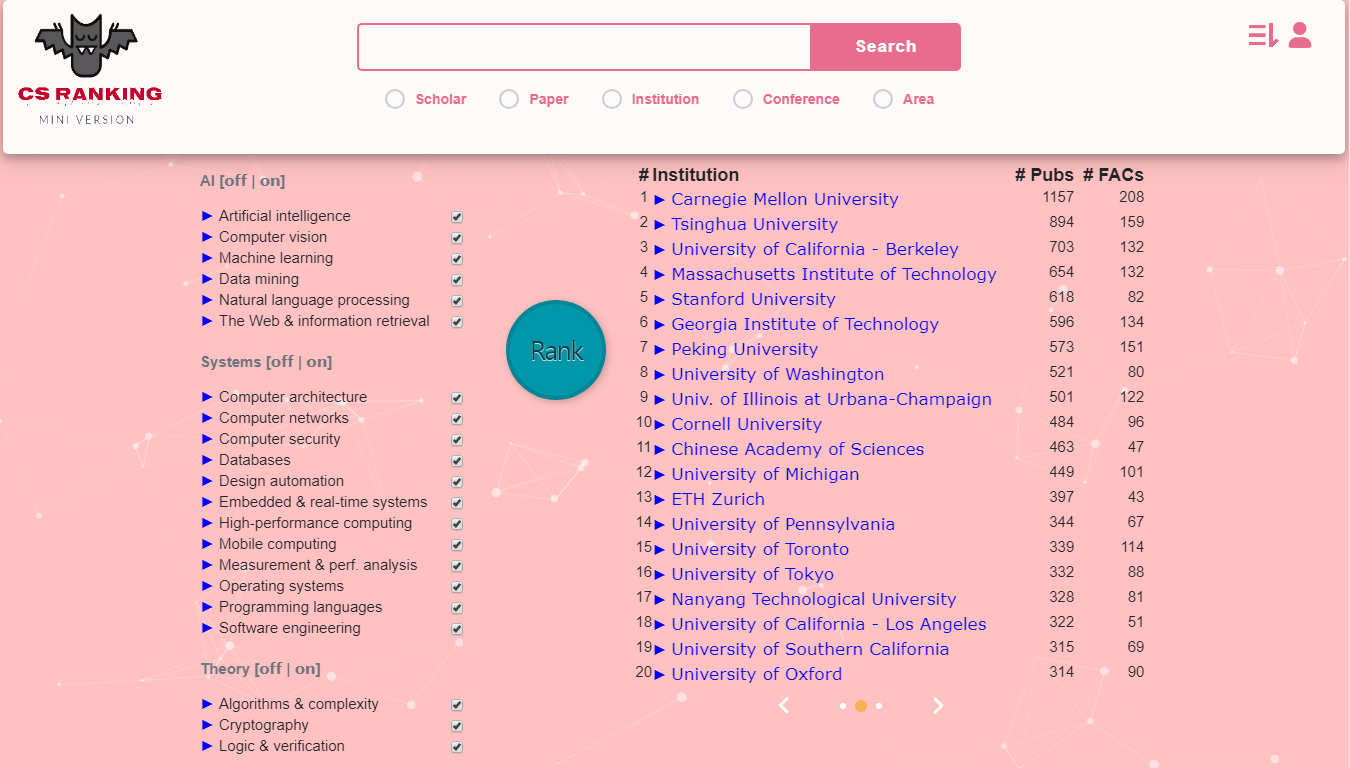
\includegraphics[width=0.8\textwidth]{asset/ranklist.png}
\end{figure}

$\quad$在排行榜中,可以看到学校的排名、发表论文数量和教师数量。点击左侧蓝色三角,即可看到学校下的老师排名。所有排名均是根据老师、学校发表的论文数量来降序排序的。老师的信息中还显示了老师所在的领域、老师的首页、老师的GoogleScholar页面和DBLP页面。

$\quad$左侧是领域的信息,点击领域旁的蓝色三角,可看到属于该领域的顶会。勾选所关心的领域,点击Rank按钮,即可在排行榜中筛选出相关领域的老师。

\item {\bf 信息检索功能}:

\begin{figure}[h]
\centering 
\subfigure{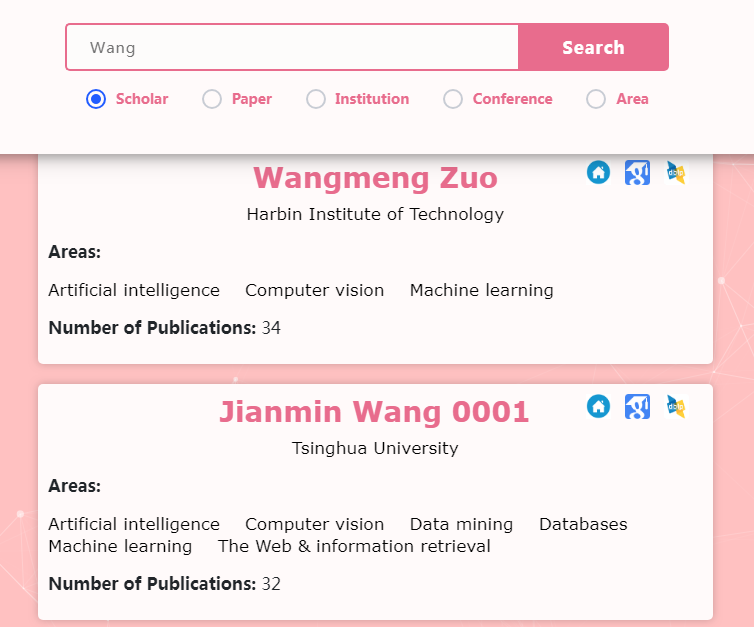
\includegraphics[width=0.4\textwidth]{asset/search_scholar.png}}
\hspace{1cm}
\subfigure{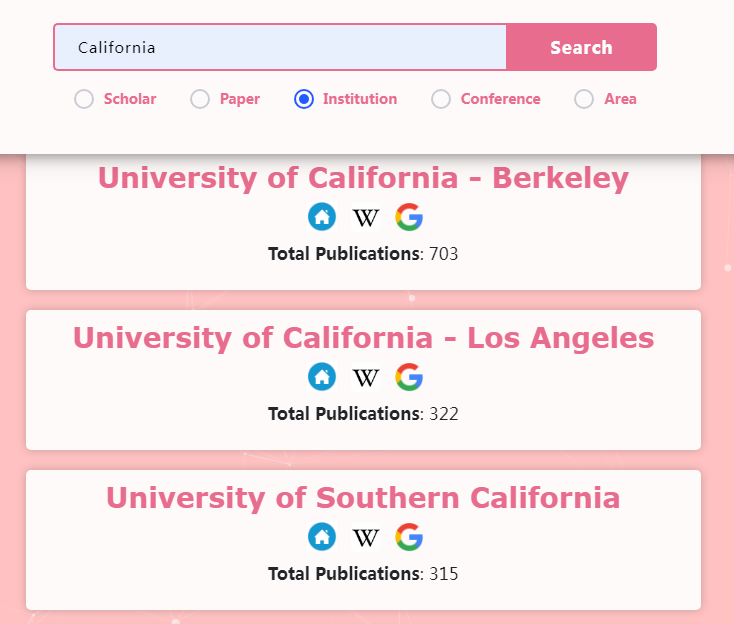
\includegraphics[width=0.4\textwidth]{asset/search_institution.png}}
\end{figure}

$\quad$为了便于检索自己感兴趣的老师,我们设计了类似GoogleScholar的搜索功能。可以通过勾选搜索框下的选项,并输入搜索关键词来检索学校、论文、老师。并且,我们为每个学校和学者都设计了自己的主页。学者的主页中包含其近几年发表的论文、每年发表的论文数量和他的合作者。学校的主页中,则详细的列举了该校的学者信息,并统计了近几年中各个领域发表论文的数量。

\item {\bf 领域会议信息}:除了上面提到的几项,我们还模仿DBLP,提供了会议和领域的检索功能,为相关领域的学者提供便利。


\begin{figure}[h]
\centering
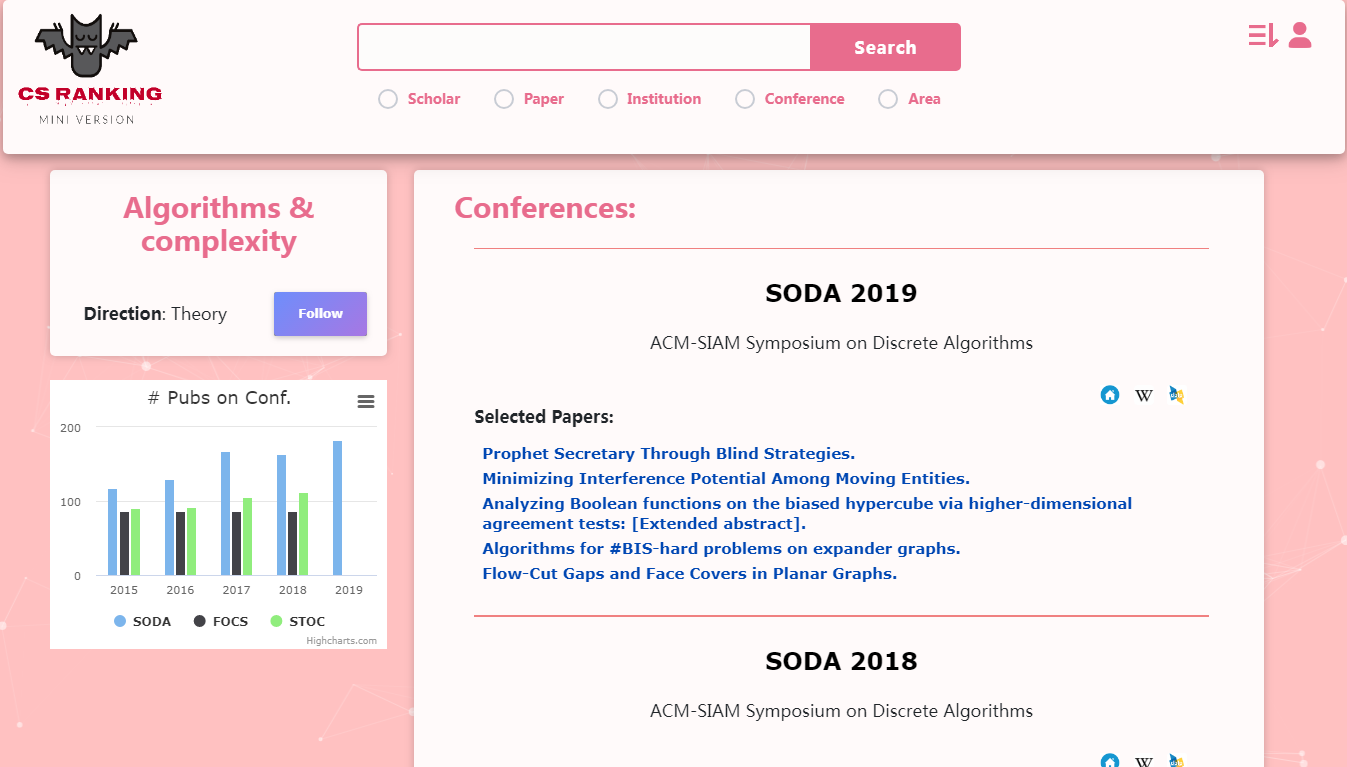
\includegraphics[width=0.75\textwidth]{asset/area.png}
\end{figure}

$\quad$在会议的相关主页中,我们给出了该会议的所有论文,并提供了访问会议首页与DBLP的链接。在领域的主页中,我们则列举了该领域的顶级会议,统计了近几年来会议中的论文数量,并给出了几位近五年来领域最活跃的学者。

\item {\bf 用户关注功能}:为了提升用户友好性,我们设计了关注功能,用户可以在相应主页关注自己感兴趣的学者、院校、领域等。这样一来,访问各主页就无需每次重新进行搜索,更加便捷;同时,当关注的学者发表新的论文时,会收到系统发来的消息提醒。

\begin{figure}[h]
\centering
\subfigure{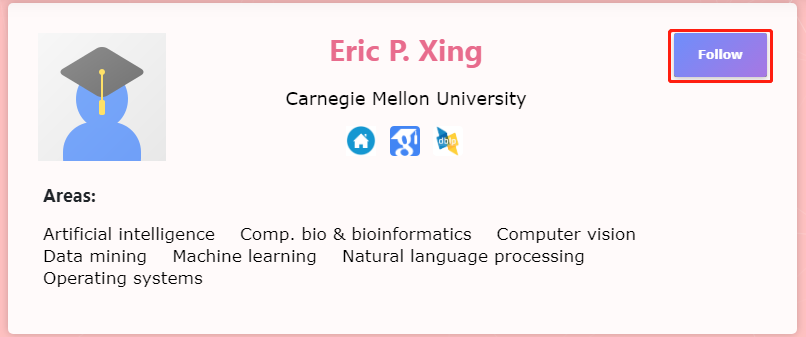
\includegraphics[width=0.6\textwidth]{asset/follow.png}}
\hspace{0.3cm}
\subfigure{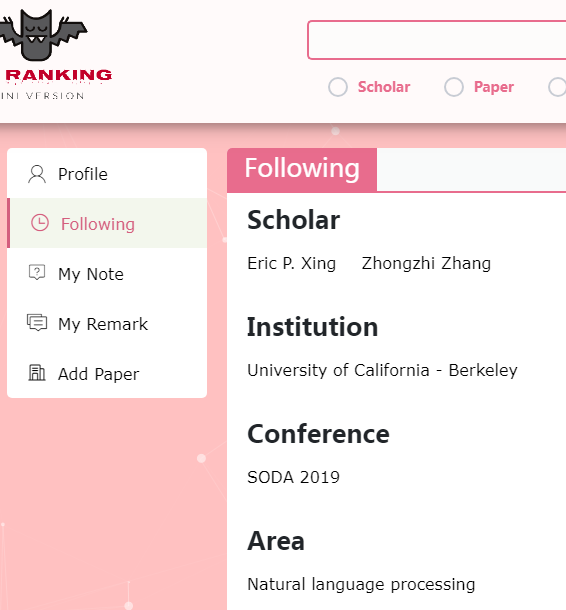
\includegraphics[width=0.35\textwidth]{asset/following.png}}
\end{figure}

\item {\bf 认证发表论文}:用户注册时,若系统检测到数据库中有姓名相似的学者,则会进行学者认证。认证后,学者的信息会自动导入用户信息中,并获得发表新论文的权限,成功发表论文后,则会通知该学者的所有关注者。

\begin{figure}[h]
\centering
\subfigure{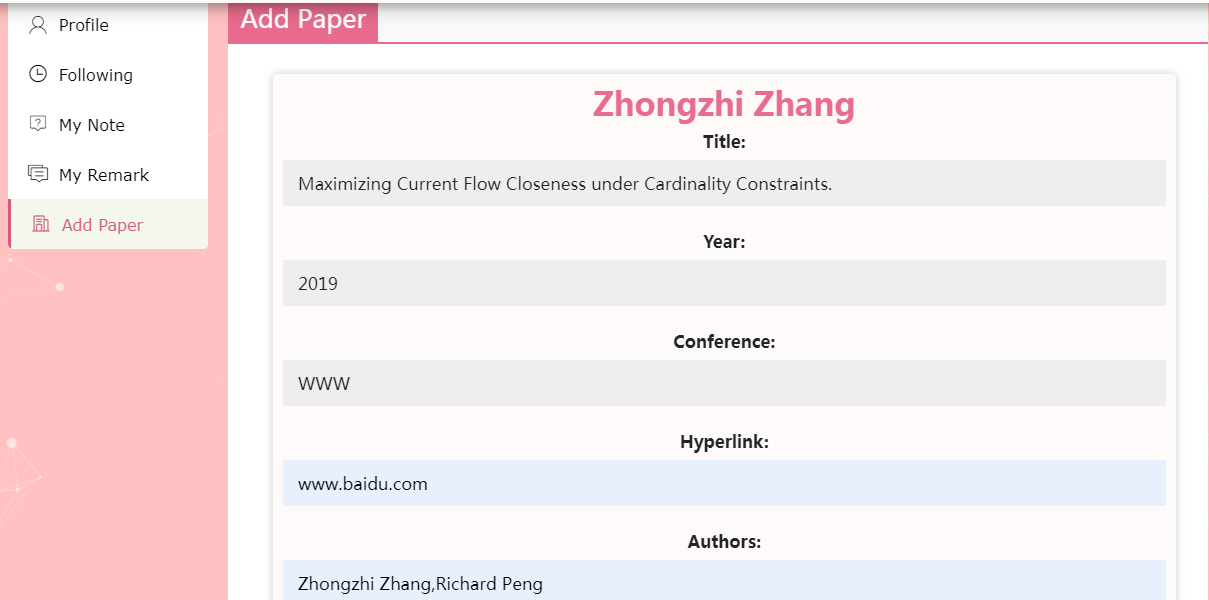
\includegraphics[width=0.6\textwidth]{asset/add_paper.png}}
\hspace{0.3cm}
\subfigure{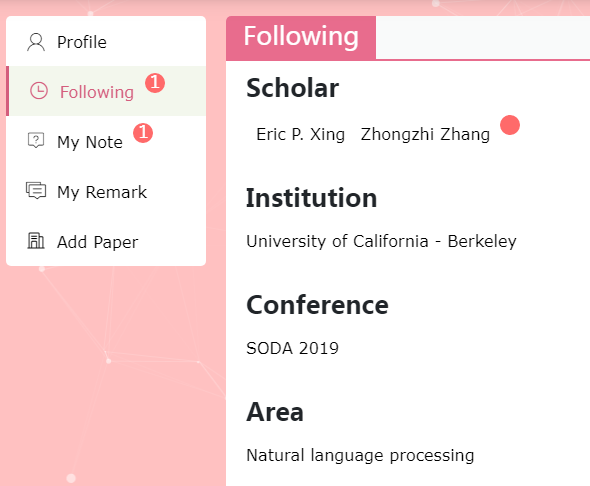
\includegraphics[width=0.35\textwidth]{asset/new_following.png}}
\end{figure}

\item {\bf 书写笔记评论}:登录后,用户可以就自己感兴趣的论文书写笔记,并会显示在论文主页下方。进入笔记主页可发表评论,笔记作者则会接收到新评论的提醒信息。

\begin{figure}[h]
\centering
\subfigure{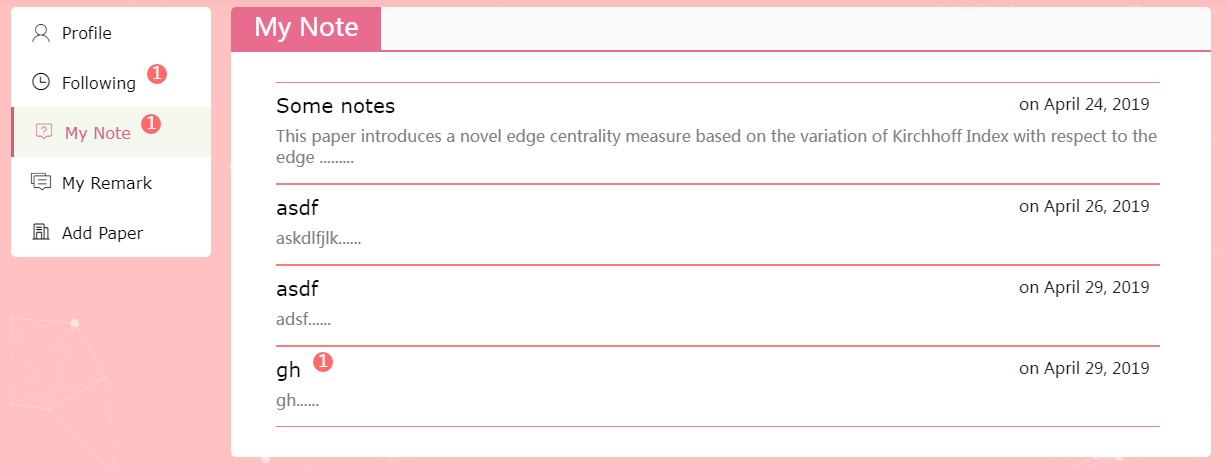
\includegraphics[width=0.9\textwidth]{asset/new_note.png}}
\end{figure}

\end{itemize}

因此,可以说,Mini-CS Ranking集合了CSRankings,GoogleScholar,DBLP三者的核心功能,又增加了友好的用户登录功能,并提供了更为美观的交互界面。



%This file contains the LaTeX code of my laboratory report for my Database course.
%Author: 周芯怡/Xinyi Zhou <17307130354@fudan.edu.cn>
%Author: 张作柏/Zuobai Zhang <17300240035@fudan.edu.cn>

\section{ER图与关系模式设计}

\subsection{ER图}

本项目设计的ER图如下:

\begin{figure}[h]
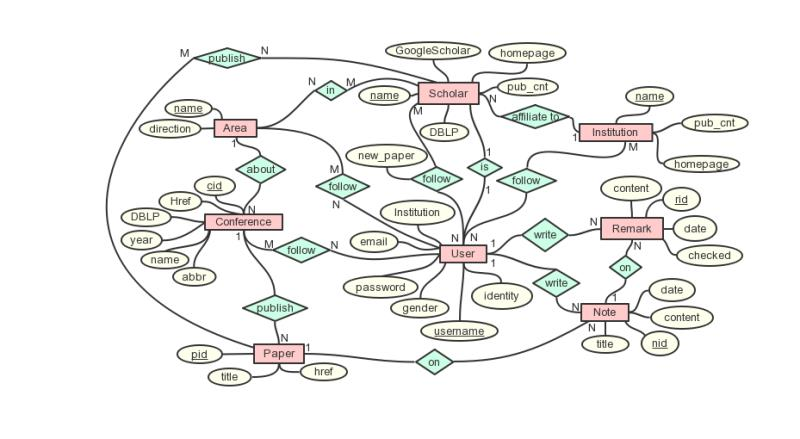
\includegraphics[width=\linewidth]{asset/ER.jpg}
\end{figure}

\subsection{关系模式与建表语句}
根据以上ER图,我们建立以下关系模式:
\begin{itemize}
\item {\myfont Institution(\uline{name}, homepage, pub\_cnt)}
\begin{lstlisting}[language=SQL]  
create table Institution(
	name char(30),
	homepage char(200),
	pub_cnt integer default 0,
	primary key(name)
	)
\end{lstlisting}
\item {\myfont Scholar(\uline{name}, homepage, DBLP, GoogleScholar, \uwave{affliliation}, pub\_cnt)}
\begin{lstlisting}[language=SQL]  
create table Scholar(
	name char(30),
	homepage  char(200),
	DBLP char(200),
	GoogleScholar char(200),
	affiliation char(30)
	pub_cnt integer default 0,
	primary key(name),
	foreign key(affiliation) references Institution(name)
	)
\end{lstlisting}
\item {\myfont Profile(\uline{username}, \uwave{scholar}, gender, identity, institution, password, email)}
\begin{lstlisting}[language=SQL]  
create table Profile(
	username char(200),
	email char(200),
	password char(200),
	scholar char(30),
	gender char(10),
	identity char(10),
	institution char(30),
	primary key(username),
	foreign key(scholar) references Scholar(name)
	)
\end{lstlisting}
\item {\myfont Conference(\uline{cid}, name, abbr, year, DBLP, Href)}
\begin{lstlisting}[language=SQL]  
create table Conference(
	cid integer,
	name char(50),
	abbr char(10),
	year integer,
	DBLP char(200),
	Href char(200),
	primary key(cid)
	)
\end{lstlisting}
\item {\myfont Paper(\uline{pid}, title, href, \uwave{conf\_id})}
\begin{lstlisting}[language=SQL]  
create table Paper(
	pid integer,
	title char(100),
	href char(500),
	conf_id integer,
	primary key(pid),
	foreign key(conf_id) references Conference(cid)
	)
\end{lstlisting}
\item {\myfont Area(\uline{name}, direction)}
\begin{lstlisting}[language=SQL] 
create table Area(
	name char(50),
	direction char(50),
	primary key(name)
	)
\end{lstlisting}
\item {\myfont Scholar\_Paper(\buline{\tuwave{scholar\_name}, \tuwave{paper\_title}})}
\begin{lstlisting}[language=SQL]  
create table Scholar_Paper(
	scholar_name char(30),
	paper_title integer,
	primary key(scholar_name, paper_title),
	foreign key(scholar_name) references Scholar(name),
	foreign key(paper_title) references Paper(pid)
	)
\end{lstlisting}
\item {\myfont Scholar\_Area(\buline{\tuwave{scholar\_name}, \tuwave{area}})}
\begin{lstlisting}[language=SQL]  
create table Scholar_Area(
	scholar_name char(30),
	area char(50),
	primary key(scholar_name, area),
	foreign key(scholar_name) references Scholar(name),
	foreign key(area) references Area(name)
	)
\end{lstlisting}
\item {\myfont Conference\_Area(\buline{\tuwave{conf\_id}, \tuwave{area}})}
\begin{lstlisting}[language=SQL]  
create table Conference_Area(
	conf_id integer,
	area char(50),
	primary key(conf_id),
	foreign key(conf_id) references Conference(cid),
	foreign key(area) references Area(name)
	)
\end{lstlisting}
\item {\myfont User\_Institution(\buline{\tuwave{user}, \tuwave{ins}})}
\begin{lstlisting}[language=SQL] 
create table User_Institution(
	user char(200),
	ins char(30),
	primary key(user, ins)
	foreign key(user) references Profile(username),
	foreign key(ins) references Institution(name)
	)
\end{lstlisting}
\item {\myfont User\_Conference(\buline{\tuwave{user}, \tuwave{conf}})}
\begin{lstlisting}[language=SQL]  
create table User_Conference(
	user char(200),
	conf integer,
	primary key(user, conf),
	foreign key(user) references Profile(username),
	foreign key(conf) references Conference(cid)
	)
\end{lstlisting}
\item {\myfont User\_Area(\buline{\tuwave{user}, \tuwave{area}})}
\begin{lstlisting}[language=SQL]  
create table User_Area(
	user char(200),
	area char(50),
	primary key(user, area),
	foreign key(user) references Profile(username),
	foreign key(area) references Area(name)
	)
\end{lstlisting}
\item {\myfont User\_Scholar(\buline{\tuwave{user}, \tuwave{sch}}, new\_paper)}
\begin{lstlisting}[language=SQL]  
create table User_Scholar(
	user char(200),
	sch char(30),
	new_paper boolean default False,
	primary key(user, sch),
	foreign key(user) references Profile(username),
	foreign key(sch) references Scholar(name)
	)
\end{lstlisting}
\item {\myfont Note(\uline{nid}, title, content, date, \uwave{author}, \uwave{paper})}
\begin{lstlisting}[language=SQL]  
create table Note(
	nid integer,
	title char(100),
	content text,
	date date,
	author char(200),
	paper integer,
	primary key(nid),
	foreign key(author) references Profile(username),
	foreign key(paper) references Paper(pid)
	)
\end{lstlisting}
\item {\myfont Remark(\uline{rid}, content, date, \uwave{author}, \uwave{note}, checked)}
\begin{lstlisting}[language=SQL]  
create table Remark(
	rid integer,
	content text,
	date date,
	author char(200),
	note integer,
	checked boolean default FALSE,
	primary key(rid),
	foreign key(author) references Profile(username),
	foreign key(note) references Note(nid)
	)
\end{lstlisting}
\end{itemize}

\subsection{函数依赖与范式分析}

{\bf 关系模式Conference}中除了非主属性对主键cid的函数依赖,还有:name→abbr,abbr→name。
形成abbr和name的传递依赖,所以只是第二范式。为了提升查询效率,我们保留了此处冗余。如果按照以下方式分解,则可以达到第三范式:\\
{\myfont Conference(name, year, DBLP, Href) \\
name\_abbr(name, abbr)}

{\bf 其余关系模式}中均只存在非主属性对主键的函数依赖,因此都是第三范式。
%This file contains the LaTeX code of my laboratory report for my Database course.
%Author: 周芯怡/Xinyi Zhou <17307130354@fudan.edu.cn>
%Author: 张作柏/Zuobai Zhang <17300240035@fudan.edu.cn>

\section{数据集获取与导入}

数据量大是本项目的特征之一,单是数据库中的论文数量就达到了5万的数量,而论文作者关系更是达到了20万的级别,而获取这些数据并导入数据库,着实花费了不少精力,因此本节将重点介绍数据集的获取过程,以及根据关系模式导入数据的流程。

本节所介绍的所有代码与文件均包含在DataProcess文件夹下,独立于整个项目。

\subsection{CS Rankings开源数据}

因为CS Rankings本身是开源项目,其数据集也是公开的\footnote{https://github.com/emeryberger/CSrankings},所以我们的一部分数据直接使用了这些开源数据,以减少工作量。

这一类数据主要包括csrankings.csv和institution.csv两个文件。csrankings.csv包含了学者姓名、所在学校、学者主页和ScholarID;institution.csv包含了学校的全称。其中学者与所在学校之间的关系,如果自己获取的话会比较麻烦。因为要到相应的学校网站上去爬取老师的数据,而这类通用性较强的爬虫是比较难做的,因此我们选择直接使用CS Rankings已经整理好的开源数据。

\subsection{DBLP开源数据集解析}

众所周知,DBLP因其便利的开源数据集而闻名,许多数据挖掘相关的研究也是在DBLP的数据集上展开的,所以我们在此就使用了DBLP的开源数据集\footnote{http://dblp.uni-trier.de/xml/},来获取论文信息与作者信息。

但是因为DBLP的数据集是xml格式,所以无法直接使用的,需要先对其进行解析。解析的代码在parser.py中,作用是将XML格式的DBLP数据集,转换为便于我们处理的paper.csv和paper\_author.csv文件。

解析的过程我们参考了https://blog.csdn.net/shuaishuai3409/article/details/54316214一文。我们调用了Python标准库中的SAX解析器进行解析,其原理是在解析XML的过程中,会触发事先由用户定义的事件。我们要做的工作就是重新定义一个xml.sax.ContentHandler的类,其中包含三种事件:
\begin{enumerate}
\item 元素开始事件startElement:遇到开始标签时触发,此时可将类中的变量清零,并记录当前标签的类别。
\item 内容处理事件characters:处理一个标签中的内容,将标签中的内容保存到局部变量中。
\item 元素结束事件endElement:遇到结束标签时触发,将局部变量中的内容保存到全局的字典中。
\end{enumerate}
需要注意的是,在处理时要区分父标签和子标签,即在父标签结束时才将局部变量清零,子标签结束时则只需要更新局部变量的属性。

因为DBLP的数据集实在太大,所以我们只取了近五年中发表在部分顶会上的论文。

具体解析过程,请参见parser.py。

\subsection{爬虫获取数据}

除去以上两个数据来源,还有一部分数据是由我们自己爬取的,例如institution\_homepage.csv,其中包含了每所学校的主页网址。

爬虫的原理是,通过一个Python脚本,不断地对某些URL发送request,接受返回的html代码,并通过分析处理获取需要的内容。为了获取每所学校的首页,我们可以在Google上搜索“CS 学校名字”,一般搜索结果的第一项就是该校计算机系的首页,因此核心思路就是:利用request向Google发送搜索请求,然后从返回的第一个搜索结果中解析出学校首页的URL。
\begin{enumerate}
\item Google提供了比较简洁的搜索URL接口:\\
https://www.google.com.hk/search?q=<keyword>\&num=1\\
表示设置搜索关键词为<keyword>,返回结果数量为1。利用Python的requests库进行访问,并通过.text属性获取html内容。
\item 对html代码的解析,我们可以先利用request获取一份html代码,并保存在本地后用浏览器打开,在调试器中找到我们想要的元素的标签。之后,我们使用了Python的BeautifulSoup库,这里我们可以很便捷地通过find方法根据标签类型和标签id找到相应元素,然后通过正则表达式进行字符串的匹配和处理。
\end{enumerate}

需要注意的是,Google的反爬虫机制做的相当智能,我们必须通过减慢访问速度和切换UserAgent来避免出现人机验证界面。

具体爬虫过程,请参见scraper.py。

\subsection{数据导入}

因为调试阶段需要多次重写数据库,而数据的导入工作又十分繁琐,所以我们自己写了一个脚本专门用于导入数据。

所有已经预处理好的数据,都在DataProcess目录下的.csv文件中。我们的任务就是从.csv文件中,按表中格式解析数据,并通过get\_or\_create方法创建新数据。这里之所以使用get\_or\_create而非create,主要是因为一次性导入全部数据耗时较长,有时我们需要多次运行脚本,而这样就有重复导入数据的情况出现,通过get\_or\_create就可以避免因为插入重复元组而报错的问题。


%This file contains the LaTeX code of my laboratory report for my Database course.
%Author: 周芯怡/Xinyi Zhou <17307130354@fudan.edu.cn>
%Author: 张作柏/Zuobai Zhang <17300240035@fudan.edu.cn>

\section{设计细节}

本节主要介绍各个页面的设计细节,包括其中涉及的难点与SQL语句。在实际的设计中,借助Django提供的便利的接口和Python对列表、字典等数据结构的支持,我们没有直接使用SQL语句进行查询以提高效率。但为了将查询功能展示得更清晰,我们还是列出所涉及的SQL语句。

\subsection{信息检索}

\subsubsection{论文主页}
我们为每篇论文设计了单独的主页,功能有显示论文作者、所属会议、所属领域:
\begin{itemize}
\item 作者:
\begin{lstlisting}[language=SQL]
select scholar_name
from Scholar_Paper
where paper_title = :pid;
\end{lstlisting}
\item 所属领域:
\begin{lstlisting}[language=SQL]
select area
from Conference_Area, Paper
where pid = :pid and Paper.conf_id = Conference_Area.conf_id;
\end{lstlisting}
\item 所属会议:因为会议是论文的一个属性,所以无需使用select语句筛选。
\begin{lstlisting}[language=SQL]
select conf_id
from Paper
where pid = :pid;
\end{lstlisting}
\end{itemize}

\subsubsection{学者主页}
\label{sec:scholar}
在每位学者的主页中,我们实现了如下功能:
\begin{itemize}
\item 显示所属学校、DBLP、GoogleScholar、Homepage等信息
\begin{lstlisting}[language=SQL]
select nameaffiliation, DBLP, GoogleScholar, homepage
from Scholar
where name = :sid;
\end{lstlisting}
\item 列举其发表的所有论文,按时间顺序降序排序,使用如下SQL语句进行查询,查询出的表记作Papers
\begin{lstlisting}[language=SQL]
select P.title, P.href, P.conf_id
from Scholar_Paper as SP, Paper as P, Conference as C
where SP.scholar_name = :sid and SP.paper_title = P.pid and P.conf_id = C.cid
order by C.year DESC;
\end{lstlisting}
\item 显示其所属领域
\begin{lstlisting}[language=SQL]
select distinct name
from Area as A, Conference_Area as CA, Papers as P
where CA.conf_id = P.conf_id and CA.area = A.name;
\end{lstlisting}
\item 显示与其合作过的学者
\begin{lstlisting}[language=SQL]
select distinct A.name
from Scholar_Paper as A, Scholar_Paper as B
where A.paper_title = B.paper_title and B.scholar_name = :sid;
\end{lstlisting}
\item 显示其近五年中每年发表的论文数量
\begin{lstlisting}[language=SQL]
select C.year, count(*)
from Scholar_Paper as SP, Paper as P, Conference as C
where SP.scholar_name = :sid and SP.paper_title = P.pid and P.conf_id = C.cid
group by C.year;
\end{lstlisting}
\item 关注功能
\begin{lstlisting}[language=SQL]
insert into User_Scholar(user, sch, new_paper)
values(:user, :sid, False);
\end{lstlisting}
\item 取消关注功能
\begin{lstlisting}[language=SQL]
delete from User_Scholar
where user = :user and sch = :sid;
\end{lstlisting}
\end{itemize}
注:在导入学者数据时,可以预先将学者的pub\_cnt计算导入。因为论文的增加和删除数量非常少,pub\_cnt很少变化,所以我们可以预先将其计算好存储起来。计算使用的SQL语句如下:
\begin{lstlisting}[language=SQL]
update Scholar
set pub_cnt = (
select count(*)
from Scholar_Paper as SP
where SP.scholar_name = Scholar.name
);
\end{lstlisting}

\subsubsection{学校主页}
\label{sec:institution}
在每所学校的主页中,我们实现了如下功能:
\begin{itemize}
\item 检索该校的所有学者,按发表论文数降序排序
\begin{lstlisting}[language=SQL]
select name
from Scholar
where affiliation = :ins
order by pub_cnt DESC;
\end{lstlisting}
\item 显示学者的基本信息。查询语句同~\ref{sec:scholar}节
\item 显示学者所属的领域。查询语句同~\ref{sec:scholar}节
\item 显示学者最近发表的几篇论文,若查询结果数目大于5,则仅取前5项。查询语句同~\ref{sec:scholar}节。
\item 统计每个领域中发表论文的数量
\begin{lstlisting}[language=SQL]
select CA.area, count(*)
from Paper as P, Conference as C, Conference_Area as CA
where P.conf_id = C.cid and CA.conf_id = C.id
group by CA.area;
\end{lstlisting}
\item 关注功能
\begin{lstlisting}[language=SQL]
insert into User_Institution(user, ins)
values(:user, :ins);
\end{lstlisting}
\item 取消关注功能
\begin{lstlisting}[language=SQL]
delete from User_Institution
where user = :user and ins = :ins;
\end{lstlisting}
\end{itemize}
注:学校的pub\_cnt不是指发表的论文数,而是每人每篇论文统计一次。也就是说,假如一篇论文中有两位来自A校的作者,那么A校的pub\_cnt会增加2。之所以这样设置,是因为考虑到每位作者对论文都有其贡献,假如A校的5位学者和B校的1位学者合著了一篇论文,那么如果说该论文对A、B校的pub\_cnt贡献都为1,未免对A校有失公平,因为A校在论文的发表中明显贡献会更大,按论文人次统计很好的解决了这一问题。

与学者的pub\_cnt类似,学校的pub\_cnt也可以在最初计算后存储。该操作涉及的SQL语句为:
\begin{lstlisting}[language=SQL]
update Insititution
set pub_cnt = (
select sum(S.pub_cnt)
from Scholar as S
where S.affiliation = Insitution.name
);
\end{lstlisting}

\subsubsection{领域主页}
在每个领域的主页中,我们实现了如下功能:
\begin{itemize}
\item 筛选该领域中的顶会
\begin{lstlisting}[language=SQL]
select conf_id
from Conference_Area
where area = :area;
\end{lstlisting}
\item 列举每个顶会的几篇论文
\begin{lstlisting}[language=SQL]
select title, href
from Paper
where conf_id = :cid;
\end{lstlisting}
\item 筛选该领域最顶尖的学者,取pub\_cnt最高的五位
\begin{lstlisting}[language=SQL]
select name, homepage, DBLP, GoogleScholar, affiliation, pub_cnt
from Scholar as S
where exists (
select *
from Scholar_Papae as SP, Paper as P, Conference as C, Conference_Area as CA
where SP.scholar_name = S.name and SP.paper_title = P.pid and P.conf_id = C.cid and CA.conf_id = C.cid and CA.area = :area
)
order by pub_cnt DESC;
\end{lstlisting}
\item 显示这些学者的相关信息,查询语句同~\ref{sec:institution}节
\item 统计每个顶会每年的论文发表量
\begin{lstlisting}[language=SQL]
select cid, count(*)
from Conference as C, Paper as P
where P.conf_id = C.cid
group by cid
\end{lstlisting}
\item 关注功能
\begin{lstlisting}[language=SQL]
insert into User_Area(user, area)
values(:user, :area);
\end{lstlisting}
\item 取消关注功能
\begin{lstlisting}[language=SQL]
delete from User_Area
where user = :user and area = :area;
\end{lstlisting}
\end{itemize}

\subsubsection{会议主页}
在每个领域的主页中,我们实现了如下功能:
\begin{itemize}
\item 列举会议基本信息
\begin{lstlisting}[language=SQL]
select name, abbr, year, DBLP, Href
from Conference
where cid = :cid;
\end{lstlisting}
\item 列举论文列表
\begin{lstlisting}[language=SQL]
select pid, title, href
from Paper
where conf_id = :cid;
\end{lstlisting}
\item 关注功能
\begin{lstlisting}[language=SQL]
insert into User_Conference(user, conf)
values(:user, :cid);
\end{lstlisting}
\item 取消关注功能
\begin{lstlisting}[language=SQL]
delete from User_Conference
where user = :user and conf = :cid;
\end{lstlisting}
\end{itemize}

\subsubsection{检索页面}

我们设计了一个搜索框,用于检索相关信息,涉及到的功能有:

{\bf 检索学者} 按照关键词检索学者,按pub\_cnt降序排序:
\begin{lstlisting}[language=SQL]
select name, homepage, DBLP, GoogleScholar, affiliation, pub_cnt
from Scholar
where name like '%<key>%'
order by pub_cnt DESC;
\end{lstlisting}

{\bf 检索论文}
\begin{lstlisting}[language=SQL]
select title, href, conf_id
from Paper
where title like '%<key>%';
\end{lstlisting}

{\bf 检索学校}
\begin{lstlisting}[language=SQL]
select name, homepage, pub_cnt
from Institution
where name like '%<key>%'
order by pub_cnt DESC;
\end{lstlisting}

{\bf 检索会议}
\begin{lstlisting}[language=SQL]
select name, abbr, year, DBLP, Href
from Conference
where name like '%<key>%' or abbr like '%<key>%';
\end{lstlisting}

{\bf 检索领域}
\begin{lstlisting}[language=SQL]
select name, direction
from Area
where name like '%<key>%';
\end{lstlisting}


\subsection{排行榜}

在ranklist.html中,我们对所有学校根据其pub\_cnt进行了排名,涉及的功能与SQL语句如下:
\begin{itemize}
\item 对所有学校按pub\_cnt降序排名
\begin{lstlisting}[language=SQL]
select name, homepage, pub_cnt
from Institution
order by pub_cnt DESC;
\end{lstlisting}
\item 统计各所学校的教职工人数
\begin{lstlisting}[language=SQL]
select I.name, count(*)
from Institution as I, Scholar as S
where I.name = S.affiliation
group by I.name;
\end{lstlisting}
\item 根据所选领域,筛选出每所学校相应的老师
\begin{lstlisting}[language=SQL]
select I.name, S.name
from Institution as I, Scholar as S
where I.name = S.affiliation and exists (
select *
from Scholar_Paper as SP, Paper as P, Conference_Area as CA
where SP.scholar_name = S.name and SP.paper_title = P.pid and P.conf_id = CA.conf_id and CA.area in :area_list
)
group by I.name;
\end{lstlisting}
\end{itemize}
注:受查询效率所限,我们没有实现按领域排名的功能,实际上这个功能的查询语句可以如下表示:
\begin{lstlisting}[language=SQL]
with Result(ins, cnt) as (
select I.name, count(*)
from Institution as I, Scholar as S, Scholar_Paper as SP, Paper as P, Conferece_Area as CA
where I.name = S.affiliation and S.name = SP.scholar_name and SP.paper_title = P.pid and P.conf_id = CA.conf_id and CA.area in :area_list
group by I.name
)
select I.name, R.cnt
from Institution as I, Result as R
where I.name = R.ins
order by R.cnt DESC;
\end{lstlisting}

\subsection{用户信息}

\subsubsection{用户个人中心}
\noindent
{\bf Profile} 显示用户的基本信息。涉及的SQL语句是:
\begin{lstlisting}[language=SQL]
select username, email, scholar, gender, identity, institution
from Profile
where username=:name;
\end{lstlisting}
{\bf Edit Profile} 提供用户修改个人信息的途径。涉及的SQL语句是:
\begin{lstlisting}[language=SQL]
update Profile
set identity=:identity, gender=:gender, email=:email, institution=:ins,password=:pw
where username=:name;
\end{lstlisting}
{\bf Follow}
\begin{itemize}
\item 显示用户关注的学者、会议、领域及机构。涉及的SQL语句有:
\begin{lstlisting}[language=SQL]
select sch
from User_Scholar
where user=:user;
select ins
from User_Institution
where user=:user;
select area
from User_Area
where user=:user;
select conf
from User_Conference
where user=:user;
\end{lstlisting}
\item 当有关注的学者发表新的论文时,会在此页面上显示提醒。涉及的SQL语句有:
\begin{lstlisting}[language=SQL]
select sch
from User_Scholar
where user=:request.user and new_paper=True;
\end{lstlisting}
\end{itemize}
{\bf My Note}
\begin{itemize}
\item 显示用户写过的所有论文笔记。涉及的SQL语句是:
\begin{lstlisting}[language=SQL]
select title, content, date
from Note
where author=:user;
\end{lstlisting}
\item 当有笔记被其他用户评论时,会在此页面上显示新消息的数量。涉及的SQL语句是:\\
统计总消息数
\begin{lstlisting}[language=SQL]
select count(*)
from Remark, Note
where Remark.note=Note.nid and Note.author=:user and checked=False;
\end{lstlisting}
统计每篇笔记消息数
\begin{lstlisting}[language=SQL]
select count(*)
from Remark
where note=:note and checked=False;
\end{lstlisting}
\end{itemize}
{\bf My Remark} 显示用户写过的所有评论
\begin{lstlisting}[language=SQL]
select content, date
from Remark
where author=:user;
\end{lstlisting}
{\bf Add Paper} 为已经认证过的用户提供添加新论文的途径。用户可以填写论文的标题、年份、会议、超链接及作者名单并提交。当用户已经通过了认证、填写的会议和学者都已经在数据库中存在并且用户是作者之一时,论文才可以添加成功。所涉及的主要SQL语句是:
\begin{itemize}
\item 更新Paper
\begin{lstlisting}[language=SQL]
insert into Paper(title, conf_id, href)
select :title, cid, :href
from Conference
where abbr=:abbr and year=:year;
\end{lstlisting}
\item 更新Schoalr\_Paper
\begin{lstlisting}[language=SQL]
insert into Scholar_Paper(scholar_name, paper_title)
values(:name, :pid);
\end{lstlisting}
\item 更新Scholar\_Area
\begin{lstlisting}[language=SQL]
insert into Scholar_Area(scholar_name, area)
select :name, area
from Conference_Area
where conf_id=:conf;
\end{lstlisting}
\item 更新User\_Scholar,使得关注学者的用户收到提醒
\begin{lstlisting}[language=SQL]
update User_Scholar
set new_paper=True
where sch=:a;
\end{lstlisting}
\item 更新论文作者的pub\_cnt
\begin{lstlisting}[language=SQL]
update Scholar
set pub_cnt = pub_cnt + 1
where name = :name;
\end{lstlisting}
\item 更新论文作者所属学校的pub\_cnt,对于每个论文作者,
\begin{lstlisting}[language=SQL]
update Insititution
set pub_cnt = pub_cnt + (
select count(*)
from Scholar
where Scholar.affiliation = Insitution.name and Scholar.name in :name_list
);
\end{lstlisting}
\end{itemize}

\subsubsection{用户登录注册}

我们实现了用户的登入、登出和注册功能,另外添加了身份认证。登入登出主要依赖Django自带的用户验证系统完成,比较简单,在此略去。

\noindent
{\bf 注册} 用户输入用户名邮箱和密码,经验证没有重名后即可注册成功
\begin{itemize}
\item 检查是否有重名
\begin{lstlisting}[language=SQL]
select conut(*)
from Profile
where username=:username;
\end{lstlisting}
\item 创建新用户
\begin{lstlisting}[language=SQL]
insert into Profile(username, email, password)
values(:username, :email, :password);
\end{lstlisting}
\end{itemize}
{\bf 认证} 注册成功后,系统会筛选姓名包含用户名的学者,让用户选择自己是否是其中之一;经过认证的用户拥有添加论文的额外权限
\begin{itemize}
\item 筛选姓名相似的学者
\begin{lstlisting}[language=SQL]
select name, affiliation
from Scholar
where name like “%:username%”;
\end{lstlisting}
\item 认证后,更新用户信息
\begin{lstlisting}[language=SQL]
update Profile
set scholar=:name, institution=:affiliation
where username=:username;
\end{lstlisting}
\end{itemize}

\subsubsection{论文及笔记}

我们为每篇论文制作了单独的主页,展示论文信息以及这篇论文的所有笔记,登陆后可以添加笔记;点击笔记进入笔记主页,展示了笔记信息和相关评论。同样,登陆后可以添加评论。

\noindent
{\bf 论文主页} 展示论文信息及笔记
\begin{itemize}
\item 筛选笔记
\begin{lstlisting}[language=SQL]
select title, content
from Note
where paper=:pid;
\end{lstlisting}
\item 添加笔记
\begin{lstlisting}[language=SQL]
insert into Note(title, content, author, paper)
values(:title, :content, :user, :paper);
\end{lstlisting}
\end{itemize}
{\bf 笔记主页} 显示笔记、评论,及添加评论
\begin{itemize}
\item 筛选笔记信息及评论
\begin{lstlisting}[language=SQL]
select Note.title, content, date, Paper.title
from Note, Paper
where Note.paper=Paper.pid and Note.nid=:nid;
select title, content, author, date
from Remark
where note=:nid
order by date desc;
\end{lstlisting}
\item 如果笔记作者是当前登录用户,笔记的所有评论设置为已读
\begin{lstlisting}[language=SQL]
update Remark
set checked=True
where note=:nid;
\end{lstlisting}
\item 添加评论
\begin{lstlisting}[language=SQL]
insert into Remark(content, author, note)
values(:content, :user, :note);
\end{lstlisting}
\end{itemize}
%This file contains the LaTeX code of my laboratory report for my Database course.
%Author: 周芯怡/Xinyi Zhou <17307130354@fudan.edu.cn>
%Author: 张作柏/Zuobai Zhang <17300240035@fudan.edu.cn>

\section{技术难点}

本节主要列举一下我们在完成项目过程中遇到的问题和所涉及的技术难点。

\begin{enumerate}
\item {\bf 网站搭建}:我们使用的是Django框架,整个网站的搭建流程如下:首先,我们在urls.py中设置好每个页面的URL网址;然后,创建若干html模板,对应于这些页面;之后,书写后端函数,通过渲染模板完成响应。为了实现各个页面之间的跳转,我们在每个页面中加入超链接,然后在访问某个页面时,通过GET请求将相应的参数传给后端。这里使用GET请求的原因是,参数可以直接在URL中看到,方便调试,也方便直接访问。

\item {\bf 字符编码}:因为在url中显示的字符会进行url编码,前后端交互时如果不进行编码和解码就会出现问题。比如当url参数中带有\&时,就必须在前端的变量后加上|urlencode;前端发送给后端的字符串,有时也需要用urllib.parse.unquote()进行解码。

\item {\bf 分页处理}:像搜索结果、排行榜之类的数据条目较多的页面,我们需要使用分页技术来控制每页显示的条目数量。这里我们使用的是Django自带的paginate方法,我们只需要传入相应的参数(进行分割的查询,每个页面的条目个数,当前是第几页)就可以接受当前页面的结果。使用Django提供的接口,这种分页方式可以不需要每次都将所有的结果都返回,而只返回需要显示的结果,大大提升了查询效率。

\item {\bf 局部刷新}:在设计follow功能时,我们在每个学者的主页添加了follow按钮。当用户未登录或未关注该学者时,按钮显示文字为follow;当用户已关注该学者时,按钮显示文字为unfollow。那么,当用户点击follow时,我们要发送请求到后端,为用户添加关注,然后将follow按钮变成unfollow选项。

这一过程看似简单,但实现起来却相当麻烦。一般而言,我们点击按钮后,会发送一个GET或POST请求给后端,后端处理后会重新渲染页面,这时网页会自动刷新。然而,整个页面的显示只有follow文字这一处发生了变化,刷新整个页面效率低下,导致使用不便捷。在这里,我们使用了{\bf jquery}的局部更新工具。

我们自行书写了一小段js代码来处理这一操作,大致思路是:首先我们为follow\_button添加事件响应函数,在follow\_button被点击时触发。接着,我们会获取按钮中文字信息,并将此作为参数,向后端发送POST请求。之后,后端处理该请求,并将相应的返回值以JSON格式传给前端。最后,前端接受后端的响应,并将相应的文字信息写入按钮中。

与之相适应的,后端的代码也需要做相应的调整:当后端接收到请求后,首先判断请求的类型是GET还是POST,若是GET,这说明是常规的请求;若是POST,则说明是点击follow按钮后,jquery发送的请求。若为POST,则首先判断用户是否登录,在根据登录情况对表进行相应修改,最后将需要在按钮中显示的信息返回。

\item {\bf 排行榜显示}:排行榜页面的显示中有三个难点:{\bf 显示/隐藏教师信息}、{\bf 自动勾选领域信息}和{\bf 排行榜的局部刷新}。
\begin{itemize}
\item 访问ranklist页面时,后端会将学校的排名连同该校老师的排名一同返回给前端,而为了不然前端显示的过于冗杂,我们默认会隐藏老师的信息。当用户点击学校旁的三角按钮时,才会显示出该校的老师。这一操作是通过html中display:none的属性完成的。在html中,将一个元素的display属性设置为none后,它将完全隐藏,不占任何位置,这样后端将老师信息传递给前端后,所有的显示任务就全部交给前端了。前端要做的就是利用js,为三角按钮设置事件,当点击该按钮时,切换老师模块的display属性,并更改三角按钮的样式。
\item 自动勾选领域信息是指,为方便用户选择领域,用户可以通过on/off按钮直接勾选/取消勾选某一方向的所有领域。这一功能利用jquery的元素选择器可以简便地完成,添加事件:当点击on时,将相应方向的每个checkbox属性都设置为勾选。
\item 排行榜的局部刷新基本原理与上一条相同。两个不同点是:1.提交POST请求时,需要获取所有checkbox的勾选状况,这个我们要通过jquery获取每个checkbox的情况写入一个数组,之后将数组作为参数传入。2.因为ranklist变化较大,所以后端返回时,我们需要按照模板将ranklist的部分重新渲染一遍,然后在前端通过.html()方法重新该部分的代码。
\end{itemize}

\item {\bf 大数据处理}:因为我们的网站中涉及的数据量较大,所以查询的效率难免会受到限制,这也是在设计网站时困扰我们的一点。一种比较合理的处理方式是,允许一些数据的冗余,比如提前计算并维护pub\_cnt这种修改次数较少,但经常被用于查询,且查询效率很低的属性。虽然会增大所占用的空间,但是考虑到其对查询效率的提升,这点空间还是值得的。
\end{enumerate}



%This file contains the LaTeX code of my laboratory report for my Database course.
%Author: 周芯怡/Xinyi Zhou <17307130354@fudan.edu.cn>
%Author: 张作柏/Zuobai Zhang <17300240035@fudan.edu.cn>

\section{外部元素}




%This file contains the LaTeX code of my laboratory report for my Database course.
%Author: 周芯怡/Xinyi Zhou <17307130354@fudan.edu.cn>
%Author: 张作柏/Zuobai Zhang <17300240035@fudan.edu.cn>

\section{结语}





\end{sloppypar}
\end{document}
